%%%%%%%%%%%%%%%%%%%%%%%%%%%%%%%%%%%%%%%%%%%%%%%%%%%%%%%%%%%%%%%%
%%                                                            %%
%% aGreekPrimer, Italian translation 2016.12 - 2017           %%
%%                                                            %%
%% From:  Clarence W. Gleason, A Greek Primer                 %%
%%        (1903, New York, American Book Company)             %%
%%                                                            %%
%%        https://archive.org/details/greekprimer00glea       %%
%%                                                            %%
%% Translated by g.p.ciceri <gp.ciceri@gmail.com>             %%
%% ---------------------------------------------------------- %%
%% This translation is Licensed under                         %%
%% Creative Commons Attribution-ShareAlike 4.0 International  %%
%% https://creativecommons.org/licenses/by-sa/4.0/            %%
%%                                                            %%
%%%%%%%%%%%%%%%%%%%%%%%%%%%%%%%%%%%%%%%%%%%%%%%%%%%%%%%%%%%%%%%%

% ᾶῖῶῆῦ  
% ἀἰὐἐὀὠἠ 
% ὰὲὶὸὺὼὴ 
% ἁἱὑὁὡἡῥ
% άέίόύήώΆΉ
% ἂἒὒἲὂὢἢὒἚἊ
% ἃἳὓὃἣὣἓἋἛ
% ἄἔἴὄὔὤἤἌἬ
% ἅἕἵὅὕὥἥἍἭ
% ἆὦἶἦὖἯἏὯἇὧἷἧὗἯἏὯ 

% ᾳῃῳ
% ᾱῑῡ
% ᾀᾐᾠ
% ᾰῐῠ
% ᾂᾒᾢ
% ϊ ϋ
% ᾄᾔᾤ
% ΰ ΐ
% ᾆᾖᾦ
% ᾲῂῲ
% ᾴῄῴ
% ᾷῇῷ
% ᾳῃῳ
% ᾱῑῡ
% ᾰῐῠ

% āēīōū
% ăĕĭŏŭ

% ᾳῃῳ
% ᾷῇῷ


\documentclass[nols]{tufte-handout}

%\geometry{showframe} % display margins for debugging page layout

\usepackage{fontspec}
\usepackage{ifxetex}
\setmainfont[Path=./fonts/palatino-linotype/, ItalicFont=palai.ttf, BoldFont=palab.ttf]{pala.ttf}


% \defaultfontfeatures{Mapping=tex-text}
% \setromanfont[Path=./fonts/TeX-Gyre-Schola/,Mapping=tex-text]{TeX Gyre Schola}
% \setsansfont[Path=./fonts/TeX-Gyre-Heros/,Scale=MatchLowercase,Mapping=tex-text]{TeX Gyre Heros}
% \setmonofont[Path=./fonts/TeX-Gyre-Cursor/,Scale=MatchLowercase]{TeX Gyre Cursor}

\usepackage{lipsum}
\usepackage{url}
\usepackage{longtable}
\usepackage{stackengine}

\usepackage{graphicx} % allow embedded images
  \setkeys{Gin}{width=\linewidth,totalheight=\textheight,keepaspectratio}
  \graphicspath{{graphics/}} % set of paths to search for images
\usepackage{amsmath}  % extended mathematics
\usepackage{booktabs} % book-quality tables
\usepackage{units}    % non-stacked fractions and better unit spacing
\usepackage{multicol} % multiple column layout facilities
\usepackage{lipsum}   % filler text
\usepackage{fancyvrb} % extended verbatim environments
  \fvset{fontsize=\normalsize}% default font size for fancy-verbatim environments

% Standardize command font styles and environments
\newcommand{\doccmd}[1]{\texttt{\textbackslash#1}}% command name -- adds backslash automatically
\newcommand{\docopt}[1]{\ensuremath{\langle}\textrm{\textit{#1}}\ensuremath{\rangle}}% optional command argument
\newcommand{\docarg}[1]{\textrm{\textit{#1}}}% (required) command argument
\newcommand{\docenv}[1]{\textsf{#1}}% environment name
\newcommand{\docpkg}[1]{\texttt{#1}}% package name
\newcommand{\doccls}[1]{\texttt{#1}}% document class name
\newcommand{\docclsopt}[1]{\texttt{#1}}% document class option name
\newenvironment{docspec}{\begin{quote}\noindent}{\end{quote}}% command specification environment

% concetti morfosintattici
\usepackage{xspace} 
\newcommand{\noun}{\textsc{sostantivo}\xspace}
\newcommand{\nouns}{\textsc{sostantivi}\xspace}
\newcommand{\adject}{\textsc{aggettivo}\xspace}
\newcommand{\adjects}{\textsc{aggettivi}\xspace}
\newcommand{\gnumber}{\textsc{numero}\xspace}
\newcommand{\gnumbers}{\textsc{numeri}\xspace}
\newcommand{\gender}{\textsc{genere}\xspace}
\newcommand{\genders}{\textsc{generi}\xspace}
\newcommand{\gcase}{\textsc{caso}\xspace}
\newcommand{\gcases}{\textsc{casi}\xspace}
\newcommand{\tense}{\textsc{tempo}\xspace}
\newcommand{\mood}{\textsc{modo}\xspace}
\newcommand{\gverb}{\textsc{verbo}\xspace}
\newcommand{\gverbs}{\textsc{verbi}\xspace}
\newcommand{\adjective}{\textsc{aggettivo}\xspace}
\newcommand{\nom}{\textsc{nom}\xspace}
\newcommand{\gen}{\textsc{gen}\xspace}
\newcommand{\dat}{\textsc{dat}\xspace}
\newcommand{\acc}{\textsc{acc}\xspace}
\newcommand{\voc}{\textsc{voc}\xspace}
\newcommand{\gexit}{\textsc{uscita}\xspace}
\newcommand{\gexits}{\textsc{uscite}\xspace}
\newcommand{\declinazione}{\textsc{declinazione}\xspace}
\newcommand{\masc}{\textsc{maschile}\xspace}
\newcommand{\femm}{\textsc{femminile}\xspace}
\newcommand{\neut}{\textsc{neutro}\xspace}

\newcommand{\indic}{\textsc{indicativo}\xspace}
\newcommand{\imper}{\textsc{imperativo}\xspace}
\newcommand{\gcong}{\textsc{congiuntivo}\xspace}
\newcommand{\ott}{\textsc{ottativo}\xspace}
\newcommand{\partic}{\textsc{participio}\xspace}
\newcommand{\infin}{\textsc{infinito}\xspace}

\newcommand{\pres}{\textsc{presente}\xspace}
\newcommand{\imperf}{\textsc{imperfetto}\xspace}
\newcommand{\aor}{\textsc{aoristo}\xspace}
\newcommand{\fut}{\textsc{futuro}\xspace}
\newcommand{\perf}{\textsc{perfetto}\xspace}
\newcommand{\pperf}{\textsc{piuccheperfetto}\xspace}

\newcommand{\sing}{\textsc{singolare}\xspace}
\newcommand{\plur}{\textsc{plurale}\xspace}
\newcommand{\dual}{\textsc{duale}\xspace}

\newcommand{\si}{\textsc{sing}\xspace}
\newcommand{\pl}{\textsc{plur}\xspace}
\newcommand{\du}{\textsc{dual}\xspace}

\newcommand{\att}{\textsc{attivo}\xspace}
\newcommand{\med}{\textsc{medio}\xspace}
\newcommand{\pass}{\textsc{passivo}\xspace}
\newcommand{\medpass}{\textsc{medio-passivo}\xspace}


% italianitudini
\renewcommand{\figurename}{Figura}
\renewcommand{\tablename}{Tabella}
\renewcommand{\contentsname}{Indice}

% fix per un qualche problema
\ifxetex
  \newcommand{\textls}[2][5]{%
    \begingroup\addfontfeatures{LetterSpace=#1}#2\endgroup
  }
  \renewcommand{\allcapsspacing}[1]{\textls[15]{#1}}
  \renewcommand{\smallcapsspacing}[1]{\textls[10]{#1}}
  \renewcommand{\allcaps}[1]{\textls[15]{\MakeTextUppercase{#1}}}
  \renewcommand{\smallcaps}[1]{\smallcapsspacing{\scshape\MakeTextLowercase{#1}}}
  \renewcommand{\textsc}[1]{\smallcapsspacing{\textsmallcaps{#1}}}
\fi

% too many float...
\extrafloats{100}

\title{A Greek Primer. Introduzione al Greco Antico \newline Lezione XIII - Il periodo ipotetico).}

\author[gpciceri]{a cura di Milagathòs: Milo's help to enjoy humanities\marginnote{\url{http://www.milagathos.com}}
}

\date{10 Gennajo 2017} % without \date command, current date is supplied


\begin{document}

\maketitle% this prints the handout title, author, and date

\begin{marginfigure}[-3.0cm]
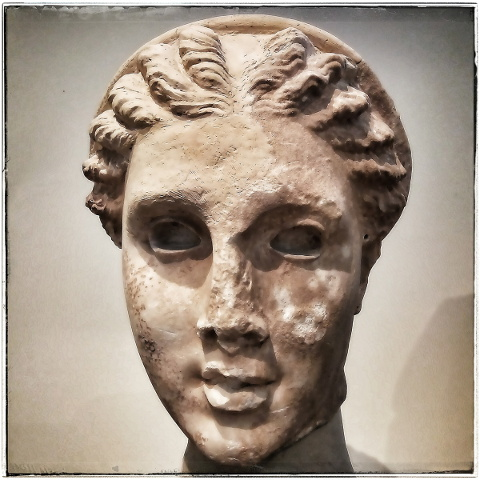
\includegraphics{smallthumb-lesson_XIII.jpeg}
\setfloatalignment{b}
\end{marginfigure}


\begin{abstract}
\noindent
Queste lezioni si articolano in \textsc{elementi grammaticali}, 
espressi sommariamente, seguiti da \textsc{vocabolari} per il lessico di base 
e da \textsc{frasi da tradurre} dal greco e in greco. 
\
L'approccio è quello del testo-laboratorio di morfosintassi: 
si presenta punto per punto - riprendendone la numerazione - 
l'esposizione di Gleason\cite{gleason1903}.\\
\bigskip
\noindent
Lezione XIII: introduzione al periodo ipotetico, vocabolario, esercizi, lettura.
\end{abstract}

%\printclassoptions

\newthought{153.} Nel periodo ipotetico, la frase che serve da condizione (la supposizione) viene detta \textbf{Protasi,}, mentre quella che fa da conclusione viene detta \textbf{Apodosi.} 

\newthought{154.} La supposizione contenuta nella protasi può essere \textit{particolare} o \textit{generale.} 
Una supposizione particolare si riferisce a un'azione \textit{definita,} che accada in un tempo \textit{definito.}
Una supposizione generale si riferisce indefinitamente a \textit{ogni azione}, che capiti \textit{in ogni tempo.}

\newthought{155.} Come avverbio di negazione, nella protasi si usa solitamente \textbf{μή,} nell'apodosi si usa invece \textbf{οὐ.} 

\newthought{156. Periodo Ipotetico Modello} da imparare a memoria:
\begin{itemize}
\item[\textsc{a.}] \textbf{εἰ γὰρ ἑκών τοῦτο πράττω, μισθὸν ἕχω,} \textit{perché se faccio questa cosa volentieri, ho una ricompensa.}
\item[\textsc{b.}] \textbf{εἰ τοῦτο ἔπραξε, καλῶς ἔχει,} \textit{se ha fatto questo, è bene.}
\item[\textsc{1.}] Osserva che in nessuno di questi due periodi si dice se la conclusione venga o meno verificata.
\item[\textsc{2.}] Osserva che i tempi verbali sono al modo indicativo in tutte e due le parti del periodo ipotetico.
\end{itemize} 

\newthought{157. Regola di sintassi} Quanto la protasi indica semplicemente una supposizione presente o passata, senza implicare nulla sulla riuscita
della condizione, si usa l'indicativo con \textbf{εἰ}. Nell'apodosi può trovarsi ogni forma verbale, ma generalmente anch'essa è all'indicativo. 

\newpage

\newthought{158. Vocabolario}

\begin{multicols}{2}
    \noindent \hangindent=1em \textbf{μισθός, ὁ} \textit{salario, paga}.  \\
    \noindent \hangindent=1em \textbf{νόμος, ὁ} \textit{legge, costume}.  \\
    \noindent \hangindent=1em \textbf{ὁπλίτης, ὁ} \textit{oplite, fante (armato in modo) pesante}.  \\
    \noindent \hangindent=1em \textbf{ὅπλον, τό} \textit{scudo;} pl. \textit{armi}.  \\
    \noindent \hangindent=1em \textbf{παρασάγγης, ὁ} \textit{parasango}, misura persiana di distanza, circa 7 Km.  \\
    \noindent \hangindent=1em \textbf{πελταστής, ὁ} \textit{peltasta, fante (armato in modo) leggero}.  \\
    \noindent \hangindent=1em \textbf{πέλτη, ἡ} \textit{scudo, bersaglio}.  \\
    \noindent \hangindent=1em \textbf{στρατιά, ἡ} \textit{esercito, armata}.  \\
    
	\noindent \hangindent=1em \textbf{ἱκανός, ή, όν} agg. \textit{sufficiente, capace}.  \\
	\noindent \hangindent=1em \textbf{ὀλίγος, η, ον} agg.  \textit{poco numeroso, pochi}.  \\
	
	\noindent \hangindent=1em \textbf{ἐξ-ελαύνω,} aor. \textbf{-ήλασα,} \textit{marciare indietro, marciare}. \\ 
	\noindent \hangindent=1em \textbf{εἰ} cong. \textit{se}.  \\
	
	\noindent \hangindent=1em \textbf{ἐνταῦθα} avv. \textit{là, a quel punto}.  \\
	\noindent \hangindent=1em \textbf{ἐντεῦθεν} avv. \textit{da quel posto, quinci}.  \\
	
	\noindent \hangindent=1em \textbf{καλῶς,} avv. \textit{bene}  \textbf{καλῶς ἔχω,} avv. \textit{sto bene} \\
	\noindent \hangindent=1em \textbf{μή} avv.neg. \textit{non}.
	
\end{multicols}

%\hyphenation{δι-δα-σκά-λου}


\newthought{159. Traduci:}
\textsc{1.}~ὁ ἄγγελος, εἰ ἔπαιε τὸν κακὸν δοῦλον, δίκαιος ἦν. \quad
\textsc{2.}~εἰ ὁ στρατηγὸς ἔφυγεν, οὐκ ἀγαθὸς ἦν μάχην. \quad
\textsc{3.}~ἐπεὶ γὰρ δείλη ἦν, οἱ πολέμιοι ἔλιπον τὰς σκηνάς. \quad
\textsc{4.}~ἐντεῦθεν ἐξ-ελαύνει δέκα παρασάγγης εἰς πεδίον καλόν. \quad
\textsc{5.}~ἐνταῦθα δὲ πολλὰς ἠμέρας ἔθυεν ἡ στρατιὰ καὶ θεοῖς καὶ θεαῖς. \quad
\textsc{6.}~οἱ σοφοὶ ἄνθρωποι τῆς κώμης γεγράφασι νόμους ἀγαθούς. \quad
\textsc{7.}~ὀλίγοι δὲ νεανίαι τῶν Περσῶν ἔπιον τὸν οἶνον. \quad
\textsc{8.}~ἱκανός γὰρ ἦν ὀ μαθητὴς δῶρα πέμπειν τῇ βασιλειᾳ. \quad
\textsc{9.}~ἐν τῷ φοβερῷ πολέμῳ οἱ στρατιῶται ἐδίωξαν τοὺς Πέρσας εἰς τὴν θάλατταν. \quad
\textsc{10.}~τῶν μὲν\sidenote{quando due parti di un periodo si corrispondono simmetricamente, si usano \textbf{μέν} e \textbf{δέ}; 
\textbf{μέν,} meglio lasciarlo non tradotto, indica che una seconda frase seguirà a quella dove compare. Le due parti sono spesso in contrapposizione.} ὀπλιτῶν τὰ ὅπλα λόγχαι ἦσαν καὶ μάχαιραι· οἱ δὲ πελτασταὶ εἶχον πέλτας μικράς.

\newthought{160. Scrivi in Greco:}
\textsc{1.}~Se non lo hai ordinato, non porteremo i regali. \quad
\textsc{2.}~Vi erano belle fonti tra gli alberi. \quad
\textsc{3.}~Se ha mandato (suo) figlio al ponte, è bene. \quad
\textsc{3.}~Il salario dei peltasti non era piccolo. \quad


\begin{figure}[!b]
  %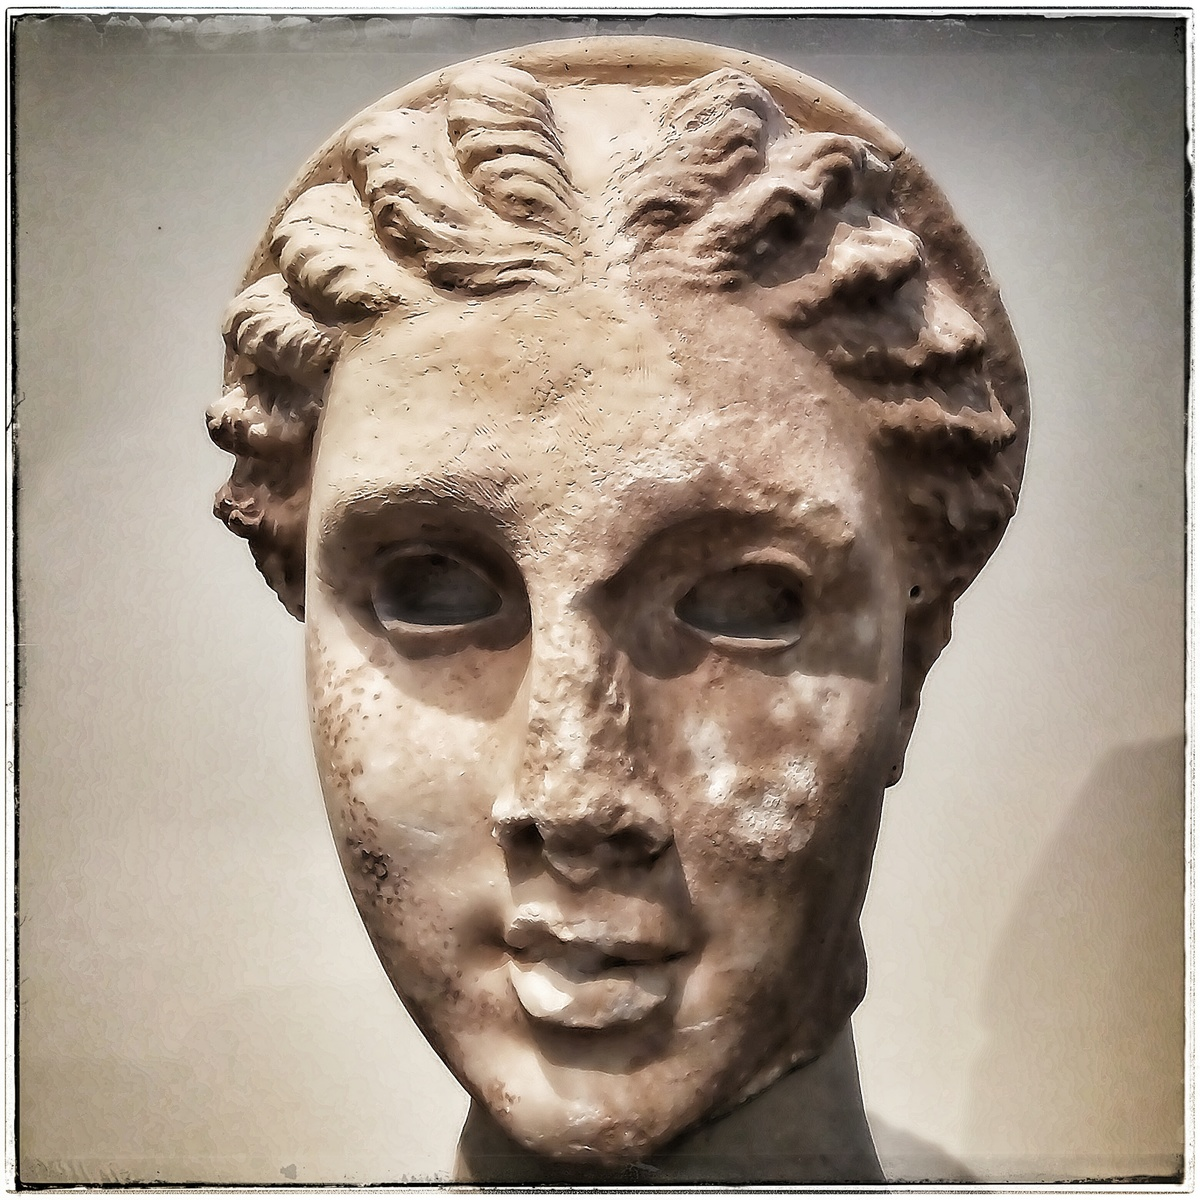
\includegraphics{thumb-lesson_XIII.jpeg}
  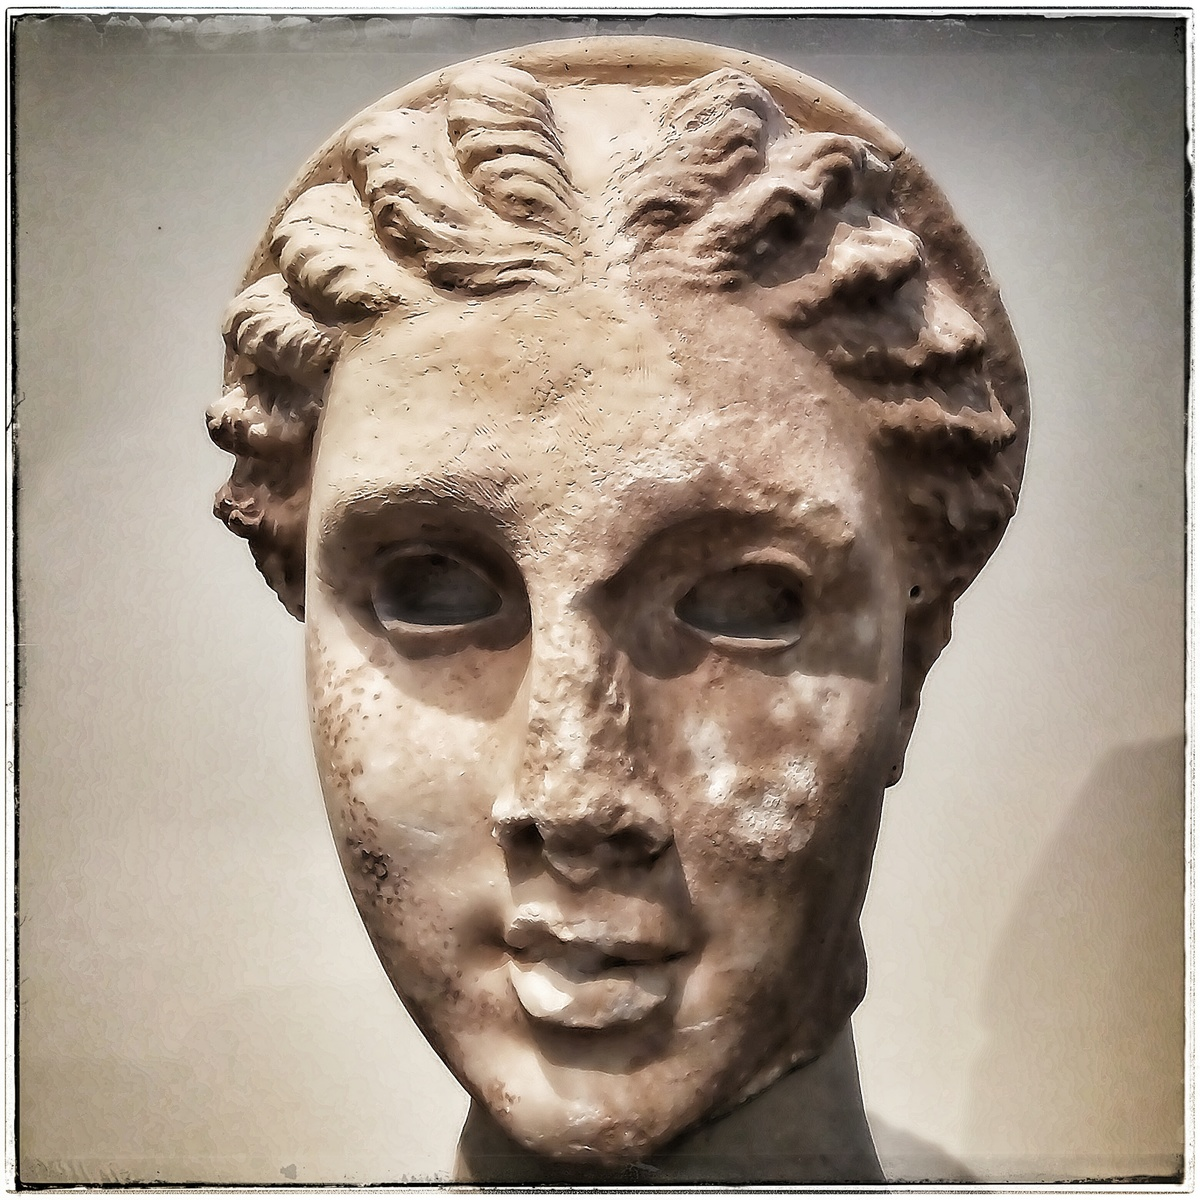
\includegraphics[width=0.5\linewidth]{thumb-lesson_XIII.jpeg}
  \caption{Museo Nazionale di Archeologia di Atene}
  \label{fig:textfig}
  %\zsavepos{pos:textfig}
  %\setfloatalignment{b}
\end{figure}

 

\nobibliography{greekBiblio}
\bibliographystyle{alpha}


\end{document}
